% =====================================================================
%  Chapitre 3 -- Classification et méthodes d'ensemble (3 h)
%  Introduction au Machine Learning -- CNFSDP -- L3 S5 -- 2026-2027
%  Version niveau licence (12/10/2026)
%  Compilation : pdflatex chapitre3.tex (deux fois)
%  Figures : code/figures_chapitre3.py
% =====================================================================
\documentclass[aspectratio=169,11pt]{beamer}
\usetheme{CNFSDP}
\usetikzlibrary{positioning,arrows.meta}
\usepackage{colortbl}

\chapitre{3}
\chapitrecourt{Ch.~3 \textendash{} Classification et ensembles}

\title{Chapitre 3 \textendash{} Classification et méthodes d'ensemble}
\subtitle{Plus proches voisins, régression logistique, arbres, forêts et boosting}
\author{Rois Céti DIMBAMBA}
\institute{Ingénieur statisticien économiste \textperiodcentered{} Actuaire \textperiodcentered{} \href{https://rdimbamba.shinyapps.io/roisceti_e-cv/}{\textcolor{cnfVert}{CV en ligne}}}
\date{?? octobre 2026}

\begin{document}

% ---------------------------------------------------------------------
\begin{frame}[plain,noframenumbering]
  \titlepage
\end{frame}

\begin{frame}{Plan et objectifs}
  \begin{columns}[T]
    \begin{column}{0.44\textwidth}
      \footnotesize\tableofcontents
    \end{column}
    \begin{column}{0.54\textwidth}
      \begin{objectifs}
        \footnotesize
        \begin{itemize}
          \item Connaître trois classifieurs : plus proches voisins, régression logistique, arbre ; les faire tourner à la main.
          \item Comprendre pourquoi une moyenne d'arbres (bagging, forêt) est plus stable qu'un arbre.
          \item Comprendre comment le boosting corrige ses erreurs pas à pas.
          \item Régler et comparer des modèles par validation croisée.
        \end{itemize}
      \end{objectifs}
      \vskip-1mm{\scriptsize\color{cnfGris}Prérequis : chapitres~1 et~2.}
    \end{column}
  \end{columns}
\end{frame}

% =====================================================================
\section{Le problème de classification}

\begin{frame}{Classer des individus}
  \begin{definition}[Problème de classification binaire]
    La cible prend deux valeurs, $y\in\{0,1\}$. On cherche un classifieur $f$ de faible probabilité d'erreur $\P\big(f(X)\ne Y\big)$.
  \end{definition}
  \vskip2mm
  {\small\textbf{Fil rouge} (chiffres fictifs) : $10$ enfants ; $x_2$ est la distance au centre de santé.}
  \vskip1mm
  \begin{center}
    \small\renewcommand{\arraystretch}{1.1}
    \begin{tabular}{lcccccccccc}
      \toprule
      enfant & 1 & 2 & 3 & 4 & 5 & 6 & 7 & 8 & 9 & 10 \\
      \midrule
      $x_1$ : années d'études de la mère & 0 & 1 & 3 & 4 & 6 & 6 & 7 & 9 & 10 & 2 \\
      $x_2$ : distance (km) & 9 & 3 & 7 & 2 & 8 & 4 & 9 & 6 & 1 & 5 \\
      $y$ : complètement vacciné & 0 & 1 & 0 & 1 & 0 & 1 & 1 & 1 & 1 & 0 \\
      \bottomrule
    \end{tabular}
  \end{center}
  {\small\color{cnfGris}Rappel du chapitre~1 : avec $\eta(x)=\P(Y=1\mid X=x)$, le meilleur classifieur prédit $1$ si $\eta(x)>\frac12$. Mais $\eta$ est inconnue.}
\end{frame}

% =====================================================================
\section{Les plus proches voisins}

\begin{frame}{La méthode des $k$ plus proches voisins}
  \begin{definition}[$k$ plus proches voisins, $k$-NN]
    Pour un nouvel individu $x$, on cherche les $k$ individus de l'échantillon les plus proches de $x$ (distance euclidienne). On estime $\eta(x)$ par la proportion de $1$ parmi eux :
    \[
      \hat\eta(x)=\frac1k\sum_{i\in V_k(x)}y_i ,
    \]
    où $V_k(x)$ est l'ensemble des $k$ voisins. On prédit la classe majoritaire chez les voisins.
  \end{definition}
  \begin{itemize}\small
    \item Aucune formule à ajuster : on garde l'échantillon et l'on compare.
    \item Distance euclidienne : $\norm{x-x_i}^2=(x_1-x_{i1})^2+\dots+(x_d-x_{id})^2$ (chapitre~0).
    \item Un seul réglage : le nombre de voisins $k$.
  \end{itemize}
\end{frame}

\begin{frame}{Le calcul sur le fil rouge}
  \small
  Nouvel enfant : mère avec $5$ ans d'études, à $5$ km du centre, $x=(5,5)$.
  \vskip1mm
  \begin{center}
    \renewcommand{\arraystretch}{1.15}\setlength\tabcolsep{5pt}
    \begin{tabular}{lcccccc}
      \toprule
      enfant & 6 & 3 & 10 & 4 & 5 & 8 \\
      \midrule
      position & $(6,4)$ & $(3,7)$ & $(2,5)$ & $(4,2)$ & $(6,8)$ & $(9,6)$ \\
      distance au carré & $1+1=2$ & $4+4=8$ & $9+0=9$ & $1+9=10$ & $1+9=10$ & $16+1=17$ \\
      vacciné & $1$ & $0$ & $0$ & $1$ & $0$ & $1$ \\
      \bottomrule
    \end{tabular}
  \end{center}
  \begin{itemize}
    \item $k=1$ : le plus proche est vacciné, $\hat\eta=1$ : on prédit \textbf{vacciné}.
    \item $k=3$ : voisins $6$, $3$, $10$, $\hat\eta=\frac13$ : on prédit \textbf{non vacciné}.
    \item $k=5$ : $\hat\eta=\frac25$ : \textbf{non vacciné}.
  \end{itemize}
  \begin{remarque}[Lecture]
    La prédiction dépend de $k$. Avec $k=1$, un seul voisin décide : la règle est très sensible au hasard de l'échantillon.
  \end{remarque}
\end{frame}

\begin{frame}{Choisir $k$, et standardiser}
  \centering
  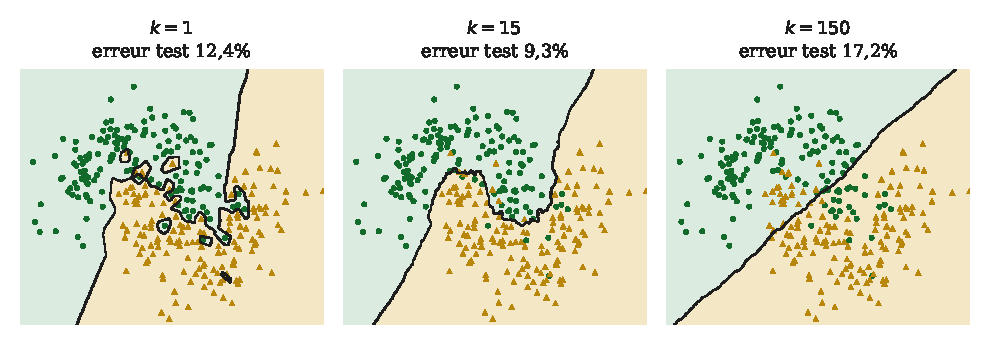
\includegraphics[width=0.74\textwidth]{knn.pdf}
  \vskip1mm
  \begin{minipage}{0.94\textwidth}
    \small
    Deux classes en « croissants » (300 points, données simulées). $k=1$ : frontière tourmentée, sur-apprentissage. $k=150$ : frontière presque droite, sous-apprentissage. On choisit $k$ par validation croisée (ici, $k=15$ convient).
    \vskip1mm
    \begin{remarque}[Standardiser]
      La distance additionne des écarts dans des unités différentes : un revenu en FCFA écraserait un nombre d'années d'études. On standardise les variables avant le $k$-NN.
    \end{remarque}
  \end{minipage}
\end{frame}

% =====================================================================
\section{La régression logistique}

\begin{frame}{Le modèle logistique}
  \begin{definition}[Régression logistique]
    On modélise la probabilité par
    \[
      \eta_\theta(x)=\sigma(\theta_0+\theta_1x_1+\dots+\theta_dx_d),\qquad\sigma(t)=\frac1{1+e^{-t}}\quad\text{(fonction \emph{sigmoïde})}.
    \]
  \end{definition}
  \centering
  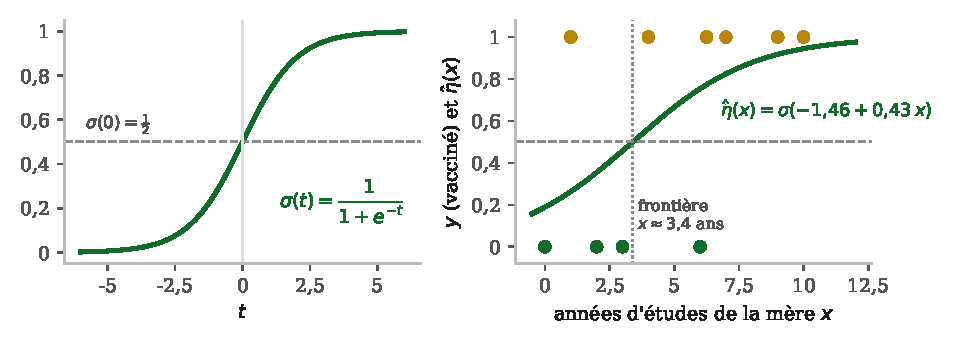
\includegraphics[width=0.7\textwidth]{sigmoide.pdf}
  \vskip-1mm
  {\small $\sigma$ croît de $0$ à $1$, avec $\sigma(0)=\frac12$. À droite : modèle ajusté sur le fil rouge (études seules).}
\end{frame}

\begin{frame}{Frontière et lecture des coefficients}
  \begin{proposition}[Frontière linéaire]
    Le classifieur logistique prédit $1$ si et seulement si $\theta_0+\theta_1x_1+\dots+\theta_dx_d>0$.
  \end{proposition}
  \begin{preuve}
    $\sigma$ est strictement croissante et $\sigma(0)=\frac12$, donc $\sigma(s)>\frac12\iff s>0$.
  \end{preuve}
  \begin{definition}[Cote]
    La \emph{cote} d'un événement de probabilité $p$ est $\frac{p}{1-p}$. Pour le modèle logistique, $\ln\frac{\eta_\theta(x)}{1-\eta_\theta(x)}=\theta_0+\theta_1x_1+\dots+\theta_dx_d$.
  \end{definition}
  \begin{exemple}[Fil rouge]
    L'ordinateur donne $\hat\theta_0=-1{,}46$ et $\hat\theta_1=0{,}43$. Frontière : $x=\frac{1{,}46}{0{,}43}\approx3{,}4$ ans d'études.
    Chaque année d'études multiplie la cote de vaccination par $e^{\hat\theta_1}\approx1{,}53$.
    Pour une mère sans instruction : $\hat\eta(0)=\sigma(-1{,}46)\approx0{,}19$ ; avec $10$ ans : $\hat\eta(10)\approx0{,}94$.
  \end{exemple}
\end{frame}

\begin{frame}{Ajuster le modèle : maximum de vraisemblance}
  \begin{definition}[Perte logistique]
    Pour une probabilité prédite $p$ et une observation $y\in\{0,1\}$ :
    $\ell(p,y)=-\big[y\ln p+(1-y)\ln(1-p)\big]$, soit $-\ln p$ si $y=1$ et $-\ln(1-p)$ si $y=0$.
  \end{definition}
  \begin{proposition}
    Maximiser la vraisemblance $\prod_i\eta_\theta(x_i)^{y_i}\big(1-\eta_\theta(x_i)\big)^{1-y_i}$ revient à minimiser la perte logistique moyenne
    $\frac1n\sum_i\ell\big(\eta_\theta(x_i),y_i\big)$.
  \end{proposition}
  \begin{preuve}
    Chaque $y_i$ suit une loi de Bernoulli de paramètre $\eta_\theta(x_i)$ (chapitre~0). Le logarithme est croissant et transforme le produit en somme : $\ln(\text{vraisemblance})=-\sum_i\ell(\eta_\theta(x_i),y_i)$.
  \end{preuve}
  {\small\color{cnfGris}La perte punit fort une confiance mal placée : prédire $p=0{,}01$ pour un enfant vacciné coûte $-\ln0{,}01\approx4{,}6$.}
\end{frame}

\begin{frame}{La perte sur le fil rouge, et le calcul de $\hat\theta$}
  \small
  Avec $\hat\theta=(-1{,}46;\,0{,}43)$ :
  \begin{itemize}
    \item enfant 4 ($x=4$, vacciné) : $\hat\eta=\sigma(0{,}26)\approx0{,}56$, perte $-\ln0{,}56\approx0{,}57$ ;
    \item enfant 5 ($x=6$, non vacciné) : $\hat\eta=\sigma(1{,}12)\approx0{,}75$, perte $-\ln0{,}25\approx1{,}40$ ;
    \item perte moyenne sur les $10$ enfants : $0{,}52$, contre $0{,}67$ pour la constante $\hat\eta=0{,}6$.
  \end{itemize}
  \vskip1mm
  \begin{proposition}[admise]
    La perte logistique moyenne est une fonction convexe de $\theta$ : elle a un seul minimum, sans formule explicite. Son gradient vaut
    \[
      \frac{\partial}{\partial\theta_j}\Big(\frac1n\sum_i\ell\Big)=\frac1n\sum_{i=1}^n\big(\eta_\theta(x_i)-y_i\big)\,x_{ij}\qquad(x_{i0}=1).
    \]
  \end{proposition}
  {\small\color{cnfGris}On le calcule par descente de gradient (chapitre~0). Le gradient est « erreur de probabilité $\times$ variable », comme pour les moindres carrés.}
\end{frame}

% =====================================================================
\section{Les arbres de décision}

\begin{frame}{L'arbre de classification}
  \begin{columns}[c]
    \begin{column}{0.44\textwidth}
      \begin{definition}[Arbre de classification]
        Un arbre pose des questions « $x_j\le s$ ? » et découpe l'espace en zones (feuilles). Dans chaque feuille, $\hat\eta$ est la proportion de $1$, et l'on prédit la classe majoritaire.
      \end{definition}
      {\small L'arbre ci-contre est appris sur le fil rouge : il classe sans erreur les $10$ enfants.}
    \end{column}
    \begin{column}{0.54\textwidth}
      \centering
      \begin{tikzpicture}[
          noeud/.style={draw=cnfVert,fill=cnfVertPale,rounded corners=1.2mm,inner sep=1.6mm,font=\small,align=center},
          feuille/.style={draw=cnfGris!60,fill=white,rounded corners=1.2mm,inner sep=1.4mm,font=\footnotesize,align=center,text width=1.9cm},
          lien/.style={-{Stealth[length=1.6mm]},draw=cnfGris,semithick},
          lab/.style={font=\scriptsize,color=cnfGris,fill=white,inner sep=1pt}]
        \node[noeud] (r) at (0,0) {distance $\le4{,}5$ km ?};
        \node[feuille] (f1) at (-1.8,-1.6) {\textbf{vacciné}\\enfants 2, 4, 6, 9\\$\hat\eta=4/4$};
        \node[noeud] (n2) at (1.7,-1.6) {études $\le6{,}5$ ans ?};
        \node[feuille] (f2) at (0.45,-3.4) {\textbf{non vacciné}\\enfants 1, 3, 5, 10\\$\hat\eta=0/4$};
        \node[feuille] (f3) at (2.95,-3.4) {\textbf{vacciné}\\enfants 7, 8\\$\hat\eta=2/2$};
        \draw[lien] (r) -- node[lab] {oui} (f1); \draw[lien] (r) -- node[lab] {non} (n2);
        \draw[lien] (n2) -- node[lab] {oui} (f2); \draw[lien] (n2) -- node[lab] {non} (f3);
      \end{tikzpicture}
    \end{column}
  \end{columns}
  \vskip2mm
  {\small\color{cnfGris}Lecture : près du centre de santé, les enfants sont vaccinés ; loin, cela dépend de l'instruction de la mère.}
\end{frame}

\begin{frame}{Choisir les questions : l'indice de Gini}
  \begin{definition}[Indice de Gini d'un groupe]
    Si une proportion $p$ du groupe est dans la classe $1$, l'\emph{impureté de Gini} du groupe est
    $G(p)=2p(1-p)$. Elle vaut $0$ pour un groupe pur ($p=0$ ou $1$) et atteint son maximum $\frac12$ pour $p=\frac12$.
  \end{definition}
  Une coupure sépare $n$ individus en deux groupes de tailles $n_g$ et $n_d$. On choisit la coupure qui minimise l'impureté moyenne
  \[
    \frac{n_g}{n}\,G(p_g)+\frac{n_d}{n}\,G(p_d).
  \]
  \begin{remarque}
    Avec $K$ classes, $G=1-\sum_kp_k^2$. On peut aussi utiliser l'entropie $-\sum_kp_k\ln p_k$ ; les deux donnent en général des arbres proches.
  \end{remarque}
\end{frame}

\begin{frame}{Le calcul sur le fil rouge}
  \small
  Avant toute coupure : $p=\frac6{10}$, $G=2\times0{,}6\times0{,}4=0{,}48$.
  \vskip1mm
  \begin{center}
    \renewcommand{\arraystretch}{1.25}
    \setlength\tabcolsep{5pt}
    \begin{tabular}{lcccccl}
      \toprule
      & \multicolumn{3}{c}{groupe « oui »} & \multicolumn{3}{c}{groupe « non »} \\
      \cmidrule(lr){2-4}\cmidrule(lr){5-7}
      coupure & effectif & $p$ & $G$ & effectif & $p$ & $G$ \\
      \midrule
      distance $\le4{,}5$ & $4$ & $1$ & $0$ & $6$ & $\frac13$ & $\frac49$ \\
      études $\le3{,}5$ & $4$ & $\frac14$ & $0{,}375$ & $6$ & $\frac56$ & $\frac5{18}$ \\
      distance $\le6{,}5$ & $6$ & $\frac56$ & $\frac5{18}$ & $4$ & $\frac14$ & $0{,}375$ \\
      \bottomrule
    \end{tabular}
  \end{center}
  Impureté moyenne : distance $\le4{,}5$ : $0{,}4\times0+0{,}6\times\frac49=\mathbf{0{,}267}$ ; les deux autres : $0{,}4\times0{,}375+0{,}6\times\frac5{18}=0{,}317$.
  On essaie toutes les coupures possibles des deux variables : la meilleure est « distance $\le4{,}5$ ».
  On recommence dans le groupe impur (« non ») : « études $\le6{,}5$ » le sépare parfaitement.
  \vskip1mm
  {\color{cnfGris}Un arbre poussé jusqu'au bout sur-apprend (chapitre~1) : on limite sa profondeur ou la taille des feuilles, réglées par validation croisée.}
\end{frame}

\begin{frame}{Forces et faiblesses d'un arbre}
  \begin{columns}[T]
    \begin{column}{0.48\textwidth}
      \textbf{Forces}
      \begin{itemize}\small
        \item Lisible : une suite de questions simples, que l'on peut expliquer.
        \item Pas besoin de standardiser ; variables qualitatives faciles.
        \item Capte des effets non linéaires et des interactions (la distance compte, puis l'instruction).
      \end{itemize}
    \end{column}
    \begin{column}{0.48\textwidth}
      \textbf{Faiblesse majeure : l'instabilité}
      \begin{itemize}\small
        \item Changer quelques individus peut changer la première question, donc tout l'arbre.
        \item Un arbre profond a une forte \emph{variance} (chapitre~1, TP1).
      \end{itemize}
    \end{column}
  \end{columns}
  \vskip3mm
  \begin{aretenir}
    Idée des méthodes d'ensemble : combiner beaucoup d'arbres. Le \textbf{bagging} fait la moyenne d'arbres instables pour réduire la variance ; le \textbf{boosting} additionne de petits arbres pour réduire le biais.
  \end{aretenir}
\end{frame}

% =====================================================================
\section{Bagging et forêts aléatoires}

\begin{frame}{Bootstrap et bagging}
  \begin{definition}[Échantillon bootstrap, bagging]
    Un \emph{échantillon bootstrap} est obtenu en tirant $n$ individus \emph{avec remise} parmi les $n$ de l'échantillon : certains apparaissent plusieurs fois, d'autres pas du tout.
    Le \emph{bagging} (\emph{bootstrap aggregating}) apprend un arbre $\hat f_b$ sur chacun de $B$ échantillons bootstrap, puis agrège :
    \[
      \hat\eta(x)=\frac1B\sum_{b=1}^B\hat\eta_b(x)\qquad\text{(ou vote majoritaire des }B\text{ arbres).}
    \]
  \end{definition}
  \begin{exemple}[Fil rouge]
    Un tirage avec remise de $10$ enfants parmi $10$ : $(3,\,7,\,7,\,1,\,9,\,4,\,4,\,4,\,10,\,6)$. Les enfants $2$, $5$ et $8$ ne sont pas tirés ; l'arbre appris sur ce tirage sera différent de celui du cours.
  \end{exemple}
\end{frame}

\begin{frame}{Pourquoi la moyenne stabilise}
  \begin{proposition}[Variance d'une moyenne]
    Si $Z_1,\dots,Z_B$ sont indépendantes, de même variance $\sigma^2$, alors $\Var\Big(\frac1B\sum_{b=1}^BZ_b\Big)=\frac{\sigma^2}{B}$.
  \end{proposition}
  \begin{preuve}
    Par indépendance, la variance d'une somme est la somme des variances (chapitre~0) : $\Var\big(\sum_bZ_b\big)=B\sigma^2$. Et $\Var(cZ)=c^2\Var(Z)$ avec $c=\frac1B$.
  \end{preuve}
  \small
  Ici $Z_b=\hat\eta_b(x)$, la prédiction du $b$-ième arbre en un point $x$. Mais les arbres sont appris sur des tirages du \emph{même} échantillon : ils sont corrélés. Si leur corrélation vaut $\rho$ (admis) :
  \[
    \Var\Big(\frac1B\sum_b\hat\eta_b(x)\Big)=\rho\,\sigma^2+\frac{(1-\rho)\,\sigma^2}{B}\;\xrightarrow[B\to\infty]{}\;\rho\,\sigma^2 .
  \]
  {\color{cnfGris}Exemple : $\sigma^2=1$, $B=100$ : variance $0{,}505$ si $\rho=0{,}5$, mais $0{,}109$ si $\rho=0{,}1$. Pour aller plus loin, il faut \emph{décorréler} les arbres.}
\end{frame}

\begin{frame}{La forêt aléatoire}
  \begin{definition}[Forêt aléatoire]
    C'est un bagging d'arbres profonds où, \emph{à chaque coupure}, l'arbre ne choisit qu'entre $m$ variables tirées au hasard parmi les $d$ (souvent $m\approx\sqrt d$).
  \end{definition}
  \begin{columns}[c]
    \begin{column}{0.5\textwidth}
      \small
      \begin{itemize}
        \item Si une variable domine, tous les arbres du bagging coupent d'abord sur elle : ils se ressemblent ($\rho$ élevé).
        \item En cachant des variables au hasard, on force des arbres variés : $\rho$ baisse, la moyenne est plus stable.
        \item Plus d'arbres ne fait pas sur-apprendre : l'erreur se stabilise.
      \end{itemize}
    \end{column}
    \begin{column}{0.48\textwidth}
      \centering
      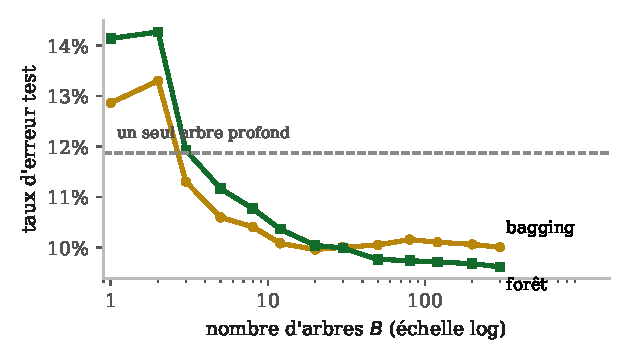
\includegraphics[width=\textwidth]{nb_arbres.pdf}
    \end{column}
  \end{columns}
\end{frame}

\begin{frame}{L'erreur out-of-bag}
  \begin{proposition}
    Dans un échantillon bootstrap de taille $n$, un individu donné n'est pas tiré avec probabilité $\big(1-\frac1n\big)^n$, qui tend vers $e^{-1}\approx0{,}37$ quand $n$ grandit (limite admise).
  \end{proposition}
  \begin{preuve}
    Chacun des $n$ tirages indépendants manque l'individu avec probabilité $1-\frac1n$.
  \end{preuve}
  {\small Pour $n=10$ : $0{,}9^{10}\approx0{,}35$. Environ un tiers des individus est \emph{hors du sac} (\emph{out-of-bag}) pour chaque arbre.}
  \begin{definition}[Erreur out-of-bag]
    Pour chaque individu $i$, on le classe en ne faisant voter que les arbres qui ne l'ont pas vu, puis on calcule le taux d'erreur sur tous les $i$.
  \end{definition}
  {\small\color{cnfGris}C'est une validation « gratuite » : elle estime l'erreur test sans mettre de données de côté.}
\end{frame}

\begin{frame}{Quelles variables comptent ?}
  \begin{definition}[Importance des variables]
    \begin{itemize}\setlength\itemsep{1pt}
      \item \textbf{Par impureté} : on additionne, sur tous les arbres, la baisse d'impureté de Gini obtenue aux coupures sur la variable $x_j$.
      \item \textbf{Par permutation} : on mélange au hasard la colonne $x_j$ dans les données test et l'on mesure la hausse de l'erreur. Si l'erreur ne bouge pas, le modèle n'utilise pas $x_j$.
    \end{itemize}
  \end{definition}
  \begin{remarque}[Précautions]
    \begin{itemize}\setlength\itemsep{1pt}
      \item Une variable importante pour le modèle n'est pas une cause : c'est une variable \emph{utile pour prédire}.
      \item Deux variables très corrélées se partagent l'importance.
      \item L'importance par permutation est plus fiable ; nous y reviendrons au chapitre~5.
    \end{itemize}
  \end{remarque}
\end{frame}

% =====================================================================
\section{Le boosting}

\begin{frame}{AdaBoost : des votes pondérés}
  Ici les classes sont codées $y\in\{-1,+1\}$ et l'on combine des arbres à une seule coupure, $h(x)\in\{-1,+1\}$.
  \begin{definition}[AdaBoost]
    Poids initiaux $w_i=\frac1n$. Pour $m=1,\dots,M$ :
    \begin{enumerate}\setlength\itemsep{1pt}
      \item choisir la coupure $h_m$ d'erreur pondérée $\varepsilon_m=\sum_{i:\,h_m(x_i)\ne y_i}w_i$ minimale ;
      \item lui donner le poids de vote $\alpha_m=\frac12\ln\frac{1-\varepsilon_m}{\varepsilon_m}$ ;
      \item multiplier $w_i$ par $e^{\alpha_m}$ si $i$ est mal classé, par $e^{-\alpha_m}$ s'il est bien classé, puis renormaliser ($\sum_iw_i=1$).
    \end{enumerate}
    Classifieur final : $\hat f(x)=\operatorname{signe}\big(\alpha_1h_1(x)+\dots+\alpha_Mh_M(x)\big)$.
  \end{definition}
  {\small\color{cnfGris}$\alpha_m>0$ dès que $\varepsilon_m<\frac12$ ; plus la coupure est bonne, plus son vote pèse.}
\end{frame}

\begin{frame}{Pourquoi le boosting change de point de vue}
  \begin{proposition}
    Après la mise à jour des poids du tour $m$, les individus mal classés par $h_m$ pèsent exactement la moitié du poids total.
  \end{proposition}
  \begin{preuve}
    Avant renormalisation, la masse des mal classés devient $\varepsilon_me^{\alpha_m}=\varepsilon_m\sqrt{\tfrac{1-\varepsilon_m}{\varepsilon_m}}=\sqrt{\varepsilon_m(1-\varepsilon_m)}$, celle des bien classés $(1-\varepsilon_m)e^{-\alpha_m}=\sqrt{\varepsilon_m(1-\varepsilon_m)}$ : les deux masses sont égales.
  \end{preuve}
  \begin{remarque}[Lecture]
    Pour les nouveaux poids, $h_m$ ne fait pas mieux que le hasard (erreur $\frac12$). Le tour suivant est donc obligé de trouver une \emph{autre} coupure, qui s'occupe des individus difficiles.
  \end{remarque}
\end{frame}

\begin{frame}{AdaBoost à la main sur six points}
  \centering
  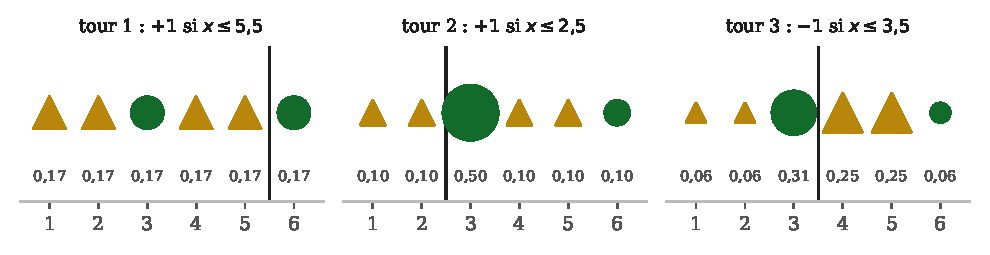
\includegraphics[width=0.84\textwidth]{adaboost.pdf}
  \vskip-1mm
  {\scriptsize\color{cnfGris}Triangles : $y=+1$ ; ronds : $y=-1$. La taille et le nombre sous chaque point donnent son poids au début du tour.}
  \vskip1mm
  \small\raggedright
  \renewcommand{\arraystretch}{1.15}
  \begin{tabular}{lcccl}
    \toprule
    tour & coupure $h_m$ & mal classés & $\varepsilon_m$ & $\alpha_m=\frac12\ln\frac{1-\varepsilon_m}{\varepsilon_m}$ \\
    \midrule
    1 & $+1$ si $x\le5{,}5$ & point 3 & $\frac16$ & $\frac12\ln5\approx0{,}80$ \\
    2 & $+1$ si $x\le2{,}5$ & points 4, 5 & $0{,}1+0{,}1=0{,}2$ & $\frac12\ln4\approx0{,}69$ \\
    3 & $-1$ si $x\le3{,}5$ & points 1, 2, 6 & $0{,}0625\times3=0{,}1875$ & $\approx0{,}73$ \\
    \bottomrule
  \end{tabular}
\end{frame}

\begin{frame}{Le vote final}
  \small
  $F(x)=0{,}80\,h_1(x)+0{,}69\,h_2(x)+0{,}73\,h_3(x)$ et $\hat f(x)=\operatorname{signe}F(x)$.
  \begin{center}
    \renewcommand{\arraystretch}{1.25}
    \begin{tabular}{ccccccc}
      \toprule
      $x$ & $y$ & $h_1$ & $h_2$ & $h_3$ & $F(x)$ & prédiction \\
      \midrule
      1, 2 & $+1$ & $+1$ & $+1$ & $-1$ & $0{,}80+0{,}69-0{,}73=0{,}76$ & $+1$ \\
      3 & $-1$ & $+1$ & $-1$ & $-1$ & $0{,}80-0{,}69-0{,}73=-0{,}62$ & $-1$ \\
      4, 5 & $+1$ & $+1$ & $-1$ & $+1$ & $0{,}80-0{,}69+0{,}73=0{,}84$ & $+1$ \\
      6 & $-1$ & $-1$ & $-1$ & $+1$ & $-0{,}80-0{,}69+0{,}73=-0{,}76$ & $-1$ \\
      \bottomrule
    \end{tabular}
  \end{center}
  \begin{aretenir}
    Chaque coupure seule se trompe sur au moins un point ; leur vote pondéré classe les six points sans erreur. Des classifieurs \emph{faibles} deviennent ensemble un classifieur \emph{fort}.
  \end{aretenir}
  {\scriptsize\color{cnfGris}scikit-learn (\texttt{AdaBoostClassifier}) affiche des poids $2\alpha_m$ : même vote, même classement.}
\end{frame}

\begin{frame}{Gradient boosting, et bilan des méthodes d'ensemble}
  \small
  \textbf{Gradient boosting en classification} : même principe qu'au chapitre~2. On part d'un score constant, et chaque petit arbre est ajusté sur les écarts $y_i-\hat\eta(x_i)$ entre la classe observée et la probabilité prédite ; on avance d'un pas $\nu$ (taux d'apprentissage).
  \vskip2mm
  \begin{center}
    \renewcommand{\arraystretch}{1.25}
    \begin{tabular}{p{0.2\textwidth}p{0.33\textwidth}p{0.36\textwidth}}
      \toprule
      & \textbf{Bagging, forêt} & \textbf{Boosting (AdaBoost, gradient)} \\
      \midrule
      Arbres & profonds, indépendants & petits, construits l'un après l'autre \\
      Agrégation & moyenne ou vote simple & somme pondérée \\
      Réduit & la variance & le biais \\
      Sur-apprend si & rarement & trop d'itérations ou $\nu$ trop grand \\
      Réglages & $B$, $m$, taille des feuilles & $M$, $\nu$, profondeur \\
      \bottomrule
    \end{tabular}
  \end{center}
\end{frame}

% =====================================================================
\section{Régler et comparer}

\begin{frame}{Des frontières très différentes}
  \centering
  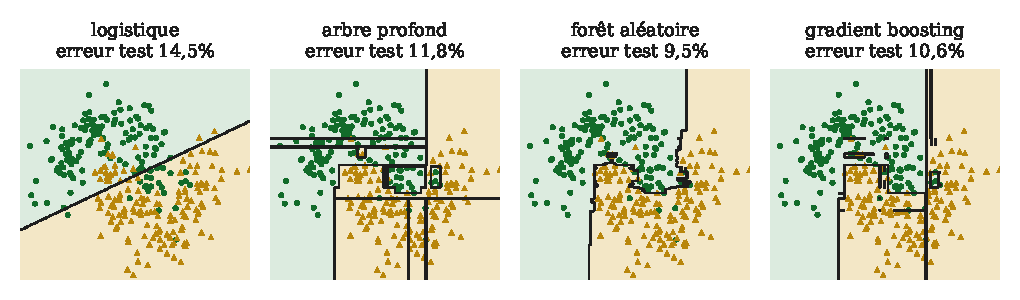
\includegraphics[width=0.94\textwidth]{frontieres.pdf}
  \vskip2mm
  \begin{minipage}{0.92\textwidth}
    \small
    Mêmes données que pour le $k$-NN. La logistique trace une droite : trop rigide pour des croissants.
    L'arbre profond découpe en rectangles et colle au bruit. La forêt et le boosting combinent des rectangles en une frontière souple et stable.
  \end{minipage}
\end{frame}

\begin{frame}{Régler les hyperparamètres par validation croisée}
  \begin{definition}[Hyperparamètre, recherche sur grille]
    Un \emph{hyperparamètre} est un réglage choisi avant l'apprentissage ($k$, profondeur, nombre d'arbres\dots). La \emph{recherche sur grille} essaie toutes les combinaisons d'une liste, estime l'erreur de chacune par validation croisée et garde la meilleure.
  \end{definition}
  \small
  \renewcommand{\arraystretch}{1.2}
  \begin{tabular}{ll}
    \toprule
    \textbf{Modèle} & \textbf{Hyperparamètres principaux} \\
    \midrule
    $k$-NN & nombre de voisins $k$ \\
    logistique & pénalité (Ridge ou Lasso, chapitre~2) \\
    arbre & profondeur maximale, taille minimale des feuilles \\
    forêt & nombre d'arbres, variables tirées $m$, taille des feuilles \\
    boosting & nombre d'arbres $M$, taux $\nu$, profondeur \\
    \bottomrule
  \end{tabular}
  \vskip2mm
  {\color{cnfGris}Le jeu test reste à l'écart de la grille : on l'utilise une seule fois, à la fin (chapitre~1).}
\end{frame}

% =====================================================================
\section{En Python}

\begin{frame}[fragile]{$k$-NN, logistique et arbre, réglés par grille}
\begin{python}[basicstyle=\ttfamily\scriptsize]
from sklearn.datasets import load_breast_cancer
from sklearn.model_selection import train_test_split, GridSearchCV
from sklearn.pipeline import make_pipeline
from sklearn.preprocessing import StandardScaler
from sklearn.neighbors import KNeighborsClassifier
from sklearn.linear_model import LogisticRegression
from sklearn.tree import DecisionTreeClassifier

X, y = load_breast_cancer(return_X_y=True)    # 569 tumeurs, 30 mesures ; y = 1 : bénigne
Xa, Xt, ya, yt = train_test_split(X, y, test_size=0.3, random_state=0, stratify=y)
knn = GridSearchCV(make_pipeline(StandardScaler(), KNeighborsClassifier()),
                   {"kneighborsclassifier__n_neighbors": [1, 3, 5, 9, 15, 25]}, cv=5)
modeles = {"k-NN": knn,
           "logistique": make_pipeline(StandardScaler(), LogisticRegression()),
           "arbre": GridSearchCV(DecisionTreeClassifier(random_state=0),
                                 {"max_depth": [1, 2, 3, 4, 6, 8, None]}, cv=5)}
for nom, f in modeles.items():
    print(nom, round(f.fit(Xa, ya).score(Xt, yt), 3))    # exactitude test
# k-NN 0.947 | logistique 0.959 | arbre 0.906   (k = 5 et profondeur 2 retenus)
\end{python}
\end{frame}

\begin{frame}[fragile]{Bagging, forêt et boosting}
\begin{python}[basicstyle=\ttfamily\scriptsize]
import numpy as np
from sklearn.ensemble import (BaggingClassifier, RandomForestClassifier,
                              AdaBoostClassifier, GradientBoostingClassifier)
souche = DecisionTreeClassifier(max_depth=1)          # arbre à une coupure
noms = load_breast_cancer().feature_names
modeles = {"arbre seul": DecisionTreeClassifier(random_state=0),
           "bagging": BaggingClassifier(DecisionTreeClassifier(),
                                        n_estimators=300, random_state=0),
           "forêt": RandomForestClassifier(n_estimators=300, oob_score=True, random_state=0),
           "AdaBoost": AdaBoostClassifier(souche, n_estimators=300, random_state=0),
           "boosting": GradientBoostingClassifier(random_state=0)}
for nom, f in modeles.items():
    print(nom, round(f.fit(Xa, ya).score(Xt, yt), 3))
foret = modeles["forêt"]
print(round(foret.oob_score_, 3), noms[np.argsort(foret.feature_importances_)[::-1][:3]])
# arbre seul 0.906 | bagging 0.93 | forêt 0.953 | AdaBoost 0.971 | boosting 0.936
# 0.967 (OOB) ['worst perimeter' 'worst radius' 'worst concave points']
\end{python}
\vskip-1mm
{\small\color{cnfGris}Sur $171$ tumeurs test, l'IC à $95\,\%$ fait environ $\pm3$ points : seul l'arbre seul est nettement derrière.}
\end{frame}

% =====================================================================
\section{TP en salle}

\begin{frame}{TP3 \textendash{} Classifieurs et méthodes d'ensemble}
  \footnotesize
  \begin{tp}{TP3 \textendash{} à faire en salle}{45 min \textperiodcentered{} \texttt{notebooks/TP3.ipynb} (Colab)}
    \begin{enumerate}\setlength\itemsep{0pt}
      \item \textbf{$k$-NN à la main} : sur le fil rouge, retrouver les prédictions du cours pour $x=(5,5)$ et $k=1,3,5$ ; vérifier avec \texttt{KNeighborsClassifier}.
      \item \textbf{Choix de $k$} : sur les croissants, tracer l'erreur de validation croisée pour $k=1,\dots,50$.
      \item \textbf{Logistique} : retrouver $\hat\theta=(-1{,}46;\,0{,}43)$ sur le fil rouge, la cote $e^{\hat\theta_1}$, et vérifier que le gradient est nul.
      \item \textbf{Gini} : écrire une fonction qui calcule l'impureté d'une coupure ; retrouver la meilleure coupure du cours.
      \item \textbf{Bagging en NumPy} : $B$ arbres sur des tirages bootstrap, vote majoritaire ; comparer à \texttt{BaggingClassifier} et à un arbre seul.
      \item \textbf{Forêt} : erreur out-of-bag contre erreur test ; trois variables les plus importantes.
      \item \textbf{AdaBoost à la main} : refaire les trois tours du cours ; comparer à \texttt{AdaBoostClassifier}.
    \end{enumerate}
  \end{tp}
\end{frame}

\begin{frame}{Résumé}
  \begin{itemize}\small
    \item Classer, c'est estimer $\eta(x)=\P(Y=1\mid X=x)$ puis seuiller (principe plug-in).
    \item $k$-NN : proportion de $1$ chez les $k$ voisins ; $k$ petit sur-apprend ; standardiser.
    \item Logistique : $\hat\eta=\sigma(\theta_0+\theta\T x)$, frontière linéaire, coefficients lus en cotes ; ajustée par maximum de vraisemblance, c'est-à-dire en minimisant la perte logistique.
    \item Arbre : questions successives choisies par l'indice de Gini ; lisible mais instable.
    \item Bagging et forêt : la moyenne de $B$ arbres divise la variance (par $B$ s'ils étaient indépendants) ; la forêt décorrèle les arbres ; erreur out-of-bag gratuite.
    \item Boosting : de petits arbres qui se concentrent sur les erreurs ; vote pondéré (AdaBoost) ou ajustement des écarts (gradient boosting).
    \item Hyperparamètres réglés par validation croisée ; comparaison finale sur le test, avec son intervalle de confiance.
  \end{itemize}
\end{frame}

\end{document}
